\section{Statistical Analysis and Modeling}
\label{sec:StatAnalisys}

The Exploratory Data Analysis conducted in previous section, hypothesis \textbf{H2} was confirmed (Due to UBER incursion in the city, the \textbf{number of trips} of yellow cabs was reduced) , and hypothesis \textbf{H4} was rejected (Due to UBER incursion in the city, the price of yellow cabs trips have decreased).

In this section we will conduct a statistical analysis to hypothesis 1 \textbf{H1} (due to UBER incursion in the city, the \textbf{travel distances} of yellow cabs trips increased), and we will provide more details to answer hypothesis 3 \textbf{H3} (The areas of the city where there is \textbf{no public transportation} coverage, correspond to areas with \textbf{low income families}). 

The notebooks used to conduct the analysis can be found in the following link: 
\href{https://marioceron-case-51.s3.amazonaws.com/datathon_html/Models_Demographics.html}{Link}


\subsection{Analysis of Hypothesis 1 \textbf{H1}. Due to UBER incursion in the city, the \textbf{travel distances} of yellow cabs trips increased}
We conducted a ttest between the distance of the trips that took place between 2014-04 and 2014-06.  The null hypothesis that is tested is that there is no change in the mean distance in both periods.

\begin{table}[h]
\begin{center}
\begin{tabular}{lclcl}
\hline
\textbf{Hypothesis Testing}  & \textbf{P-Value}   \\
\hline
Green Cabs rush & 0.0 \\
 Green Cabs weekends  &  0.0  \\
Green Cabs  & 0.0078 \\
\hline
\end{tabular}
\caption{ttest Green cabs.}
\label{tab:ttestGreen}
\end{center}
\end{table}


From Table \ref{tab:ttestGreen}, we can conclude that the null hypothesis is rejected. 

\begin{table}[h]
\begin{center}
\begin{tabular}{lclcl}
\hline
\textbf{Hypothesis Testing}  & \textbf{P-Value}   \\
\hline
Yellow Cabs weekends/weekday & 0.181 \\
Yellow Cabs rush-non rush-non	  &  0.905  \\
\hline
\end{tabular}
\caption{ttest Yellow cabs.}
\label{tab:ttestYellow}
\end{center}
\end{table}

From Table \ref{tab:ttestYellow}, we can conclude that we fail to reject the null hypothesis. There is no enough statistical evidence to assert that the distance of the trips that took
place between 2014-04 and 2014-06 is DIFFERENT from the ones between 2015-04 and 2015-06.



\subsection{Analysis of Hypothesis 3 \textbf{H3} The areas of the city where there is \textbf{no public transportation} coverage, correspond to areas with \textbf{low income families} 
}

The maps created in Section \ref{secc:heatMaps} provided a clue of the behaviour in each NTA of the different analyzed trasnportation options. The variable ``yellow\_indicator" was created. It allows us to know in which NTAs, public transportation has not an adequate coverage, or in which ones public transportation is not commonly used. Both analyzed with the total number of trips per NTA. Details of how this variable was created are provided in Section \ref{subsubsec:featureEng}.

With the variable ``yellow\_indicator" defined per NTA (1 if not many trips started in that NTA, otherwise 0), demographic information was analyzed to know if there is a pattern in the income of the people that live in those areas. Figure \ref{fig:incomesNTA} shows the violin and box plots of the mean income vs the indicator of used of public transportation. From the plots we can see that most of the people that do not frequently use public transportation, do correspond to people with high incomes. Both plots show that we have some outliers in the data, that could lead to miss-interpretation of the information. In the areas where people use public transportation more frequently, live people with very high incomes.  

Excluding people with very high incomes from the analysis, we can reject the stated hypothesis. Digging into more details, we found that the people with the highest rent live in Manhattan, which correspond to one of the areas where public transportation is commonly used.

\begin{figure}%
\centering
\subfigure[Violin plot ]{%
\label{fig:heatMapTotalPickDrop_a}%
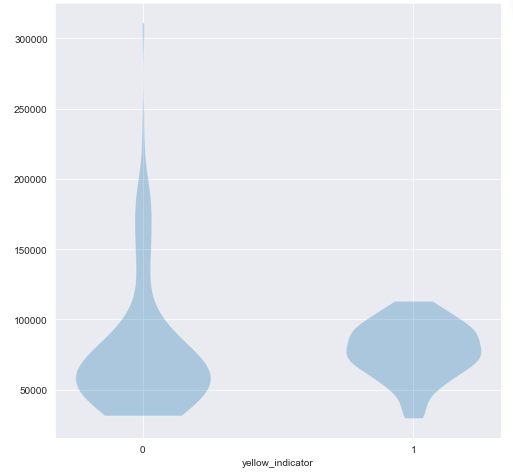
\includegraphics[height=3in, width=3in]{violinMeanIncome.png}}
\qquad
\subfigure[Box plot ]{%
\label{fig:heatMapTotalPickDrop_b}%
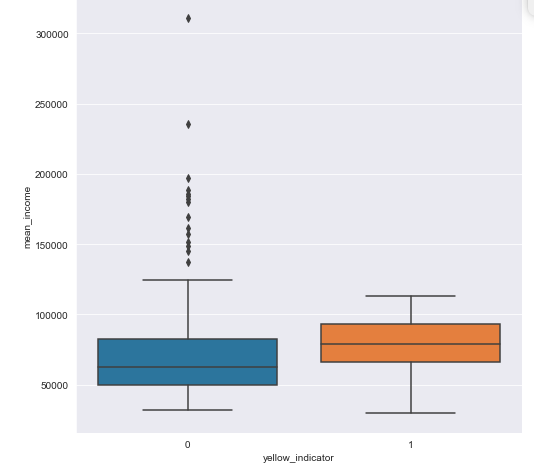
\includegraphics[height=3in, width=3in] {boxplotMeanIncome.png}}
\caption{Analyzing Mean income between NTAs that frequently use public transportation (yellow indicator = 0) vs. the ones that do not frequently use it  (yellow indicator = 1)}
\label{fig:incomesNTA}%
\end{figure}



Finally, Figure \ref{fig:age_incomesNTA} shows the comparison between the different age ranges and income ranges of the NTAs that have a yellow\_indicator = 0 and yellow\_indicator = 1. From the figure we can see the following pattern of people that live in the NTAs with yellow indicator = 1 :

\begin{itemize}
\item Most of the people that live in those areas are adults over 40 years old, some families with children.
\item Most of them with higher incomes ($50000<$ incomes $< 200.000$ USD) than the ones that live in the zones with yellow\_indicator = $0$. Excluding the ones with incomes $> 200.000$

\end{itemize}

 
\begin{figure}%
\centering
\subfigure[Distribution of age between the NTAs with yellow\_indicator = 0 and yellow\_indicator = 1]{%
\label{fig:heatMapTotalPickDrop_a}%
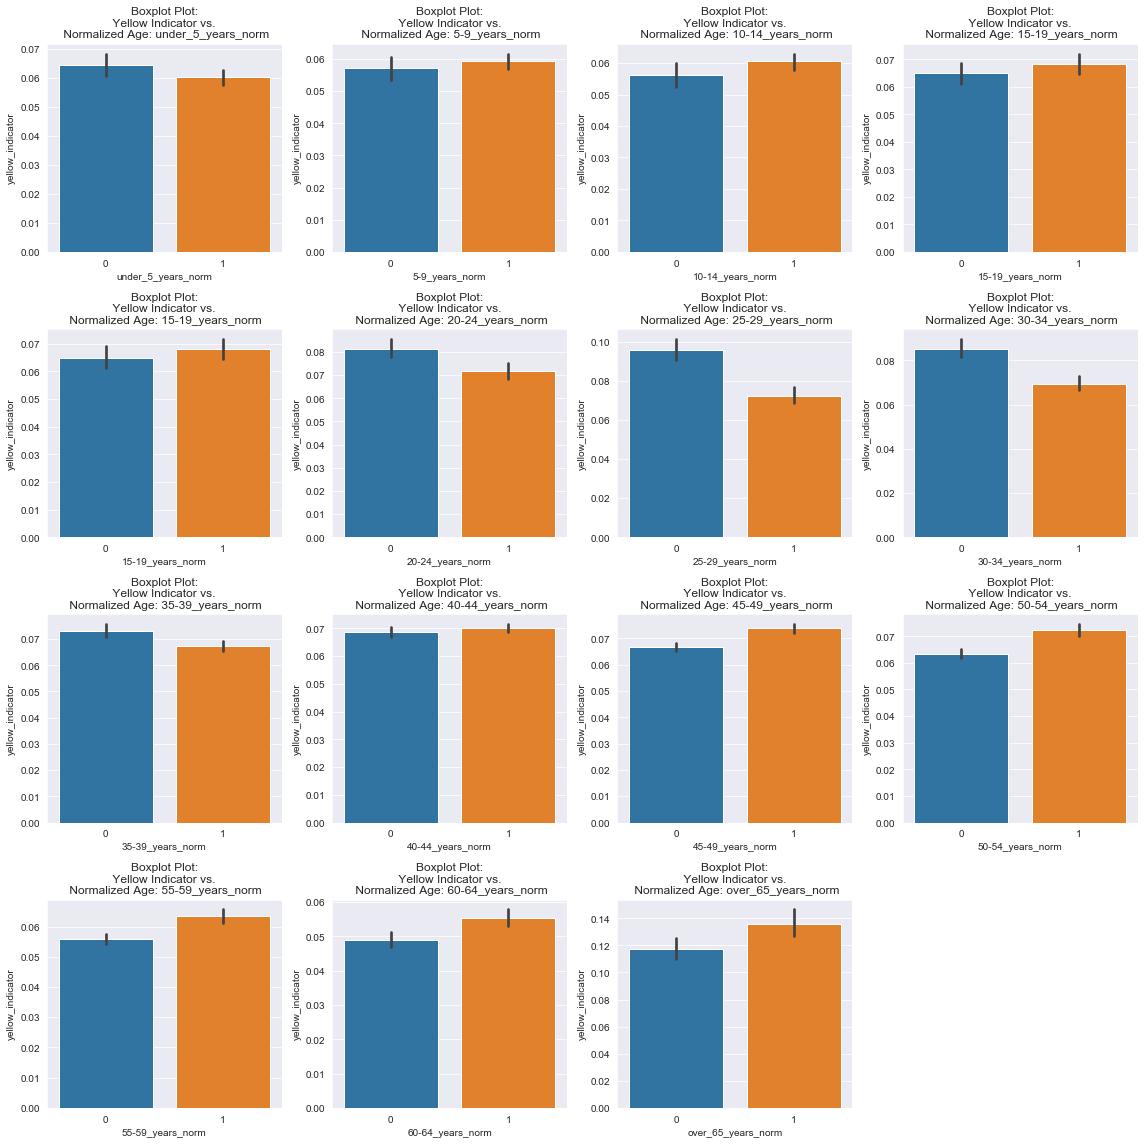
\includegraphics[height=4in, width=7in]{age_norm}}
\qquad
\subfigure[Distribution of income between the NTAs with yellow\_indicator = 0 and yellow\_indicator = 1]{%
\label{fig:heatMapTotalPickDrop_b}%
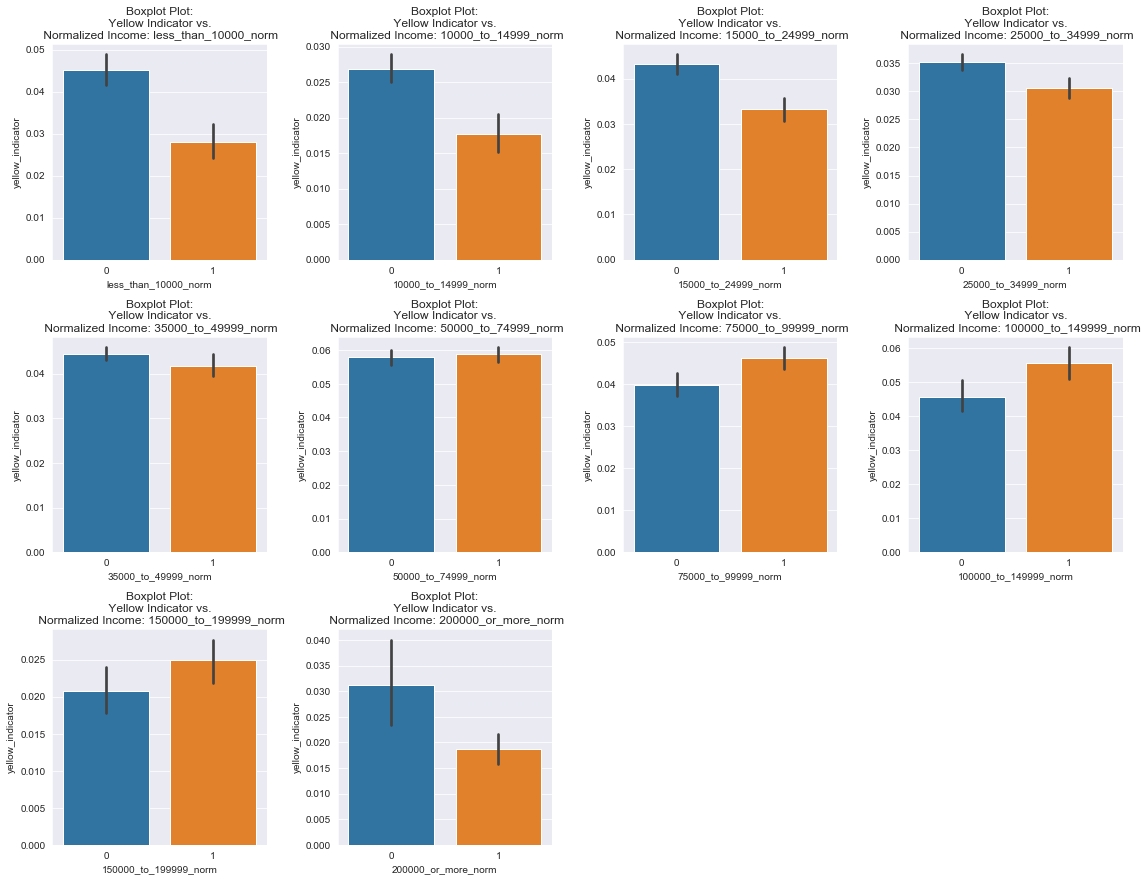
\includegraphics[height=4in, width=7in] {income_norm}}
\caption{Analyzing the behaviour of age and income between the the NTAs with yellow\_indicator = 0 and yellow\_indicator = 1}
\label{fig:age_incomesNTA}%
\end{figure}


\subsection{Model fitting}

We fit a model a random forest to predict the Yellow Indicator, based on some demographic information. The idea was to be able to create a model trained with data from 2014 and 2015 that could be used to create a new map projected in 2019. The latter with the aim of analyzing if \textbf{no changes} are done in terms of mobility, and population grows and demographic information changes, how do those changes affect the coverage. 

The model was created with the following variables. The dependent variable is the yellow\_indicator. The independent variables the different age ranges (normalized by population), and the different income ranges (normalized by population). The data was split 70\% for training and 30\% for testing. We obtain an 87.72\% of accuracy and 82.35\% of precision. Figure \ref{fig:randomForest} shows a histogram of the results with the test set. The histogram was created plotting the differences between the real values and the predicted  ones. 

\begin{figure}%
\centering
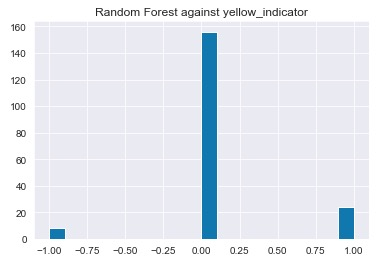
\includegraphics[height=2.5in, width=4in]{random_forest_yellow-indicator.jpg}
\caption{Random forest predictions for the yellow\_indicator. The plot shows the differences between the real values and the predicted ones.}
\label{fig:randomForest}%
\end{figure}

